% ============================================================
% ============================================================
% NACA0012 -- CONVECTIVE HEAT TRANSFER
% ============================================================
% ============================================================

\section[HTC $\&$ Thermodynamic]{\textbf{Convective Heat Transfer}}

% ============================================================
% ONERA M6 -- Convective Heat-Transfer Distribution
% ============================================================

\begin{frame}[shrink]{\small ONERA M6 -- Convective Heat-Transfer Distribution (L1)}
\scriptsize

% ------------------------------------------------------------
% Middle slice -- 1 mm roughness
% ------------------------------------------------------------
\only<1>{
\centering
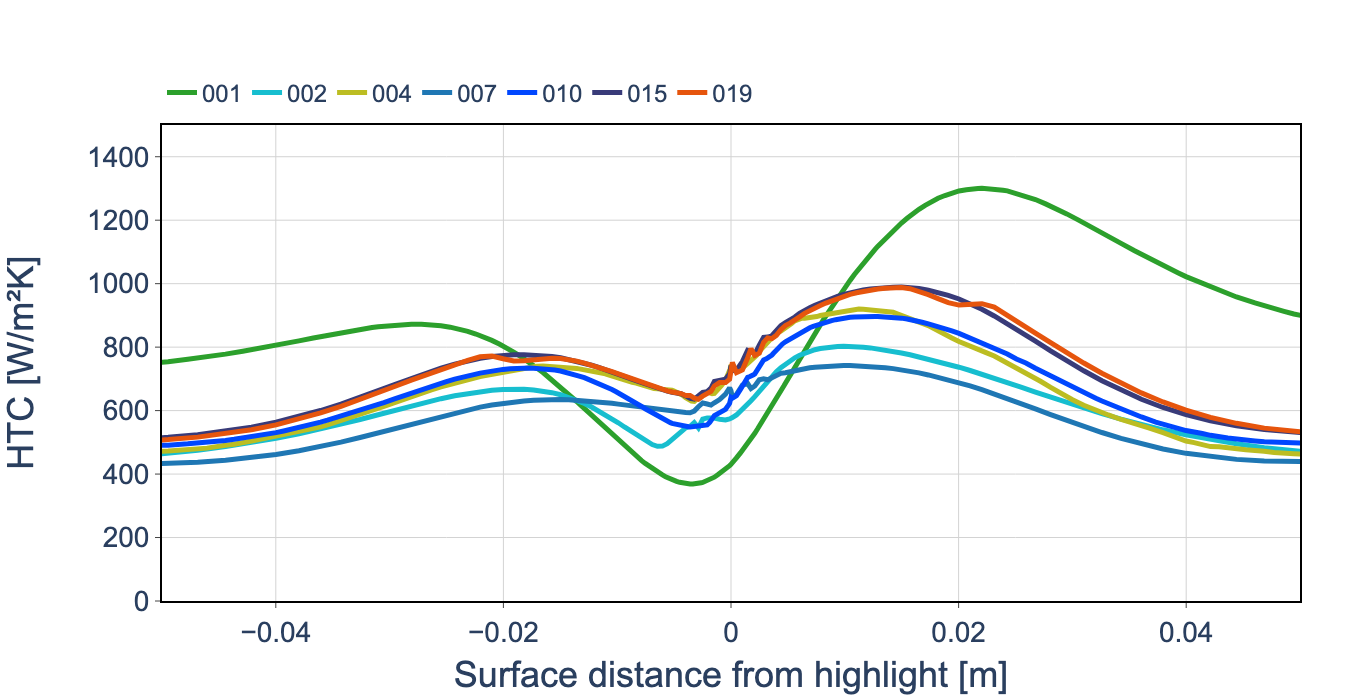
\includegraphics[width=0.5\textwidth]{FIGURES/HTC/tc_oneram6_L1_htc_vs_s_slice_0p75_roughness_1mm.png}

\vspace{0.05cm}

\textbf{$y=0.75$ m}
}

% ------------------------------------------------------------
% Inboard and outboard slices -- 1 mm roughness
% ------------------------------------------------------------
\only<2>{
\begin{columns}[T,onlytextwidth]

\begin{column}{0.50\textwidth}
    \centering
    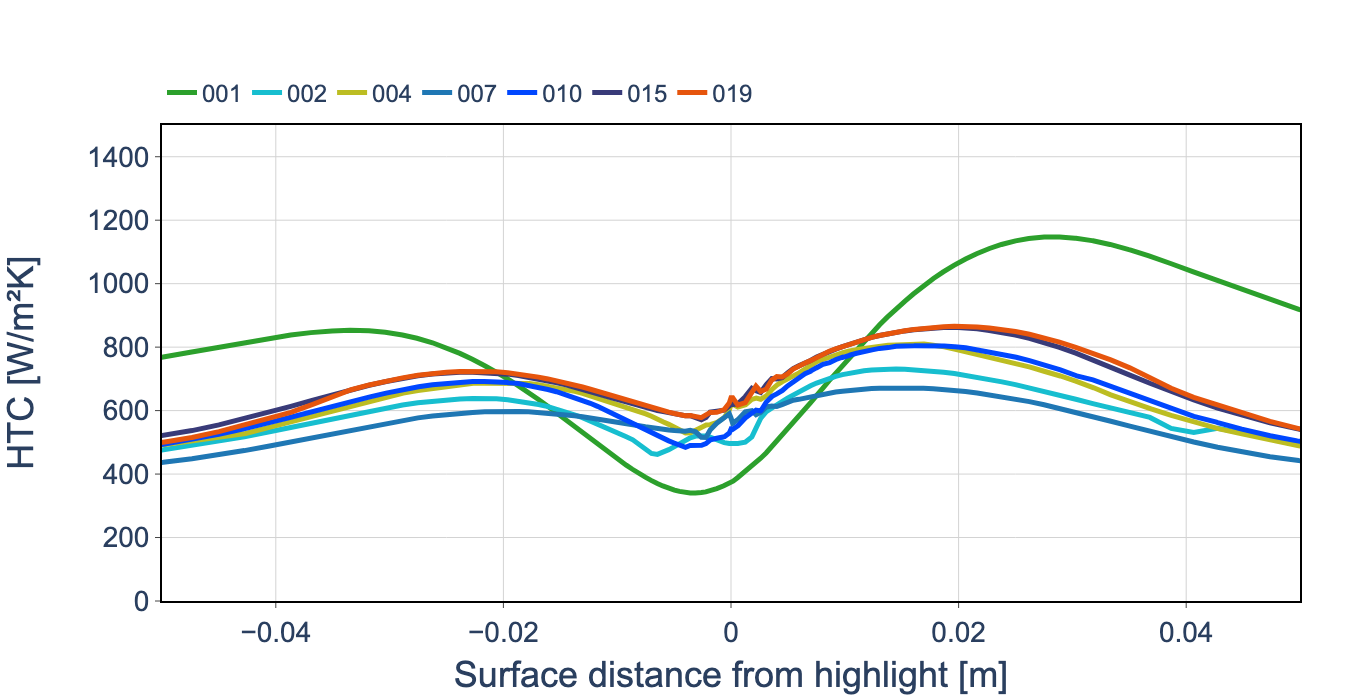
\includegraphics[width=0.94\textwidth]{FIGURES/HTC/tc_oneram6_L1_htc_vs_s_slice_0p1_roughness_1mm.png}

    \vspace{0.05cm}

    \textbf{$y=0.10$ m}
\end{column}

\begin{column}{0.50\textwidth}
    \centering
    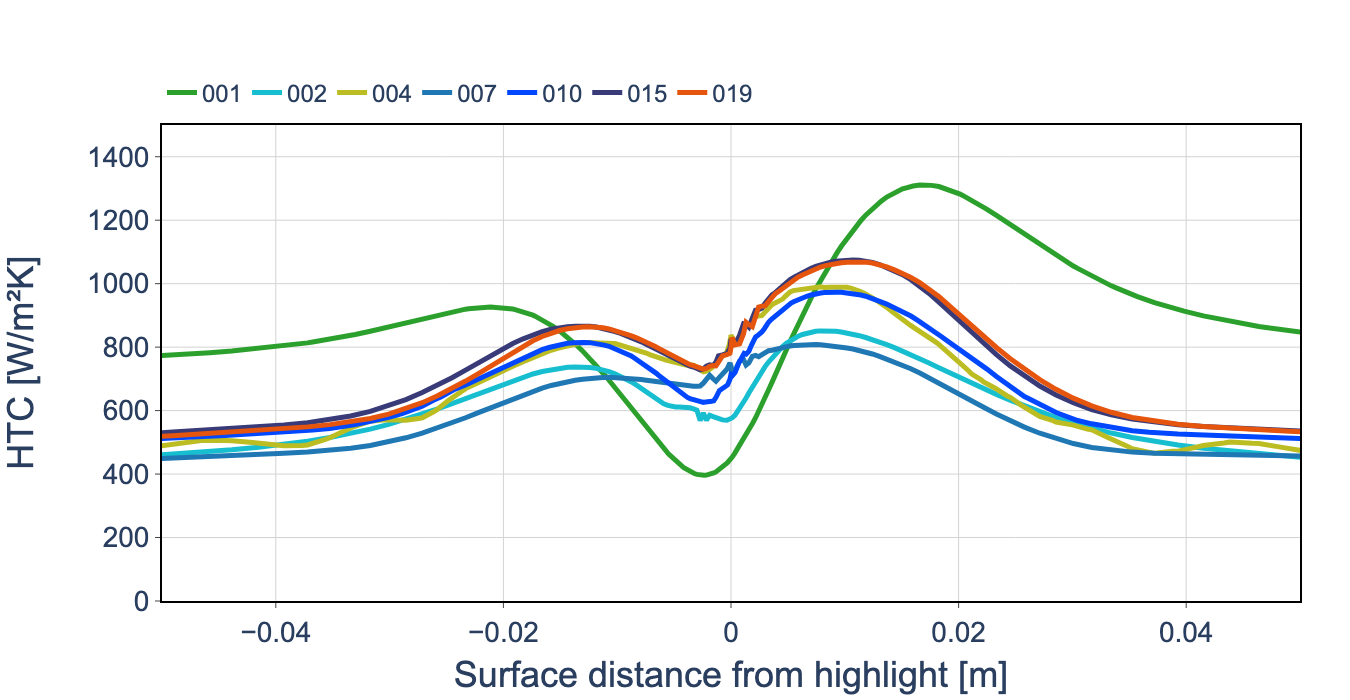
\includegraphics[width=0.94\textwidth]{FIGURES/HTC/tc_oneram6_L1_htc_vs_s_slice_1p4_roughness_1mm.png}

    \vspace{0.05cm}

    \textbf{$y=1.40$ m}
\end{column}

\end{columns}
}

% ------------------------------------------------------------
% Middle slice -- grouped by roughness
% ------------------------------------------------------------
\only<3>{
\centering
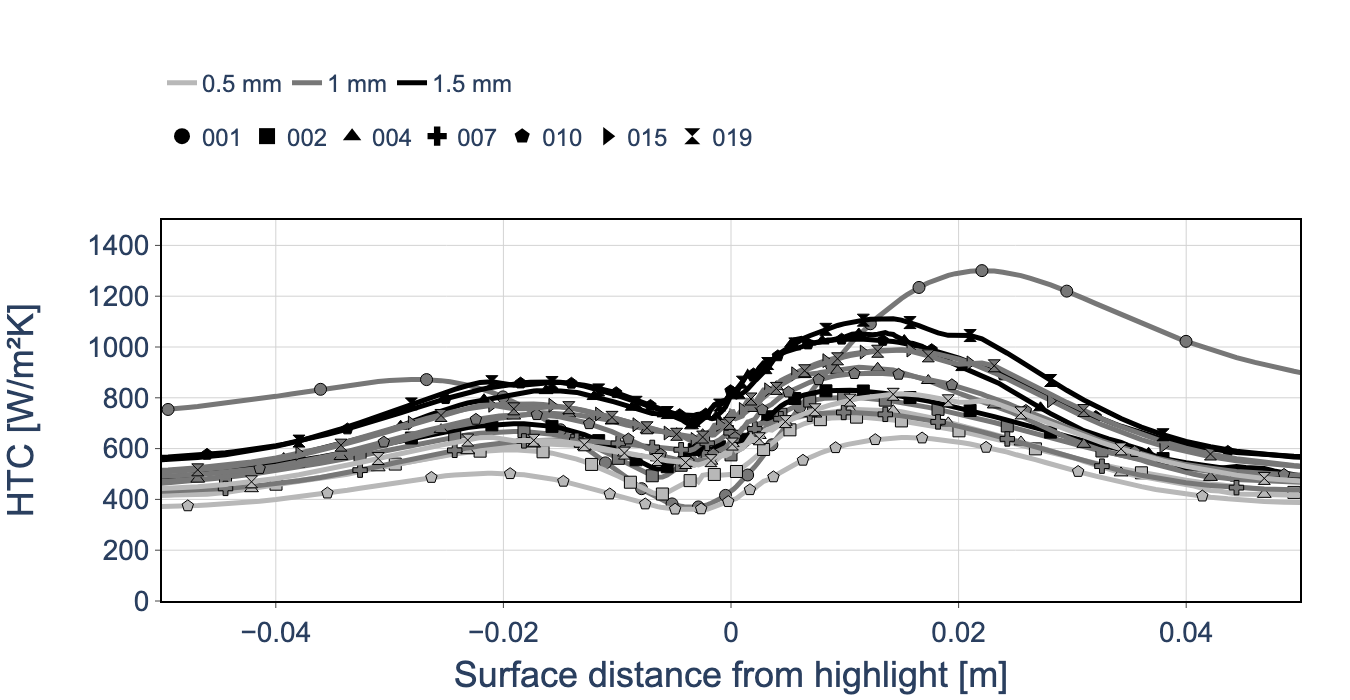
\includegraphics[width=0.62\textwidth]{FIGURES/HTC/tc_oneram6_L1_htc_vs_s_slice_0p75_all_roughness.png}

\vspace{0.05cm}

\textbf{$y=0.75$ m}
}

\vspace{0.10cm}

\begin{block}{\scriptsize Observations}
\begin{itemize}
    \item<1-> At the prescribed $1$ mm roughness, considerable code-to-code differences are observed in $HTC$, particularly near the leading edge.
    \item<2-> Similar variability is observed at the other spanwise stations, indicating that roughness alone does not explain the code-to-code scatter.
    \item<3-> Increasing roughness generally increases the predicted $HTC$, although the magnitude of the roughness effect varies between codes.
\end{itemize}
\end{block}

\end{frame}


% ============================================================
% ONERA M6 -- Participant-Level Roughness Sensitivity
% ============================================================

\begin{frame}{\small ONERA M6 -- Participant-Level HTC Roughness Sensitivity (L1)}
\scriptsize
\vspace{-0.2cm}
\centering
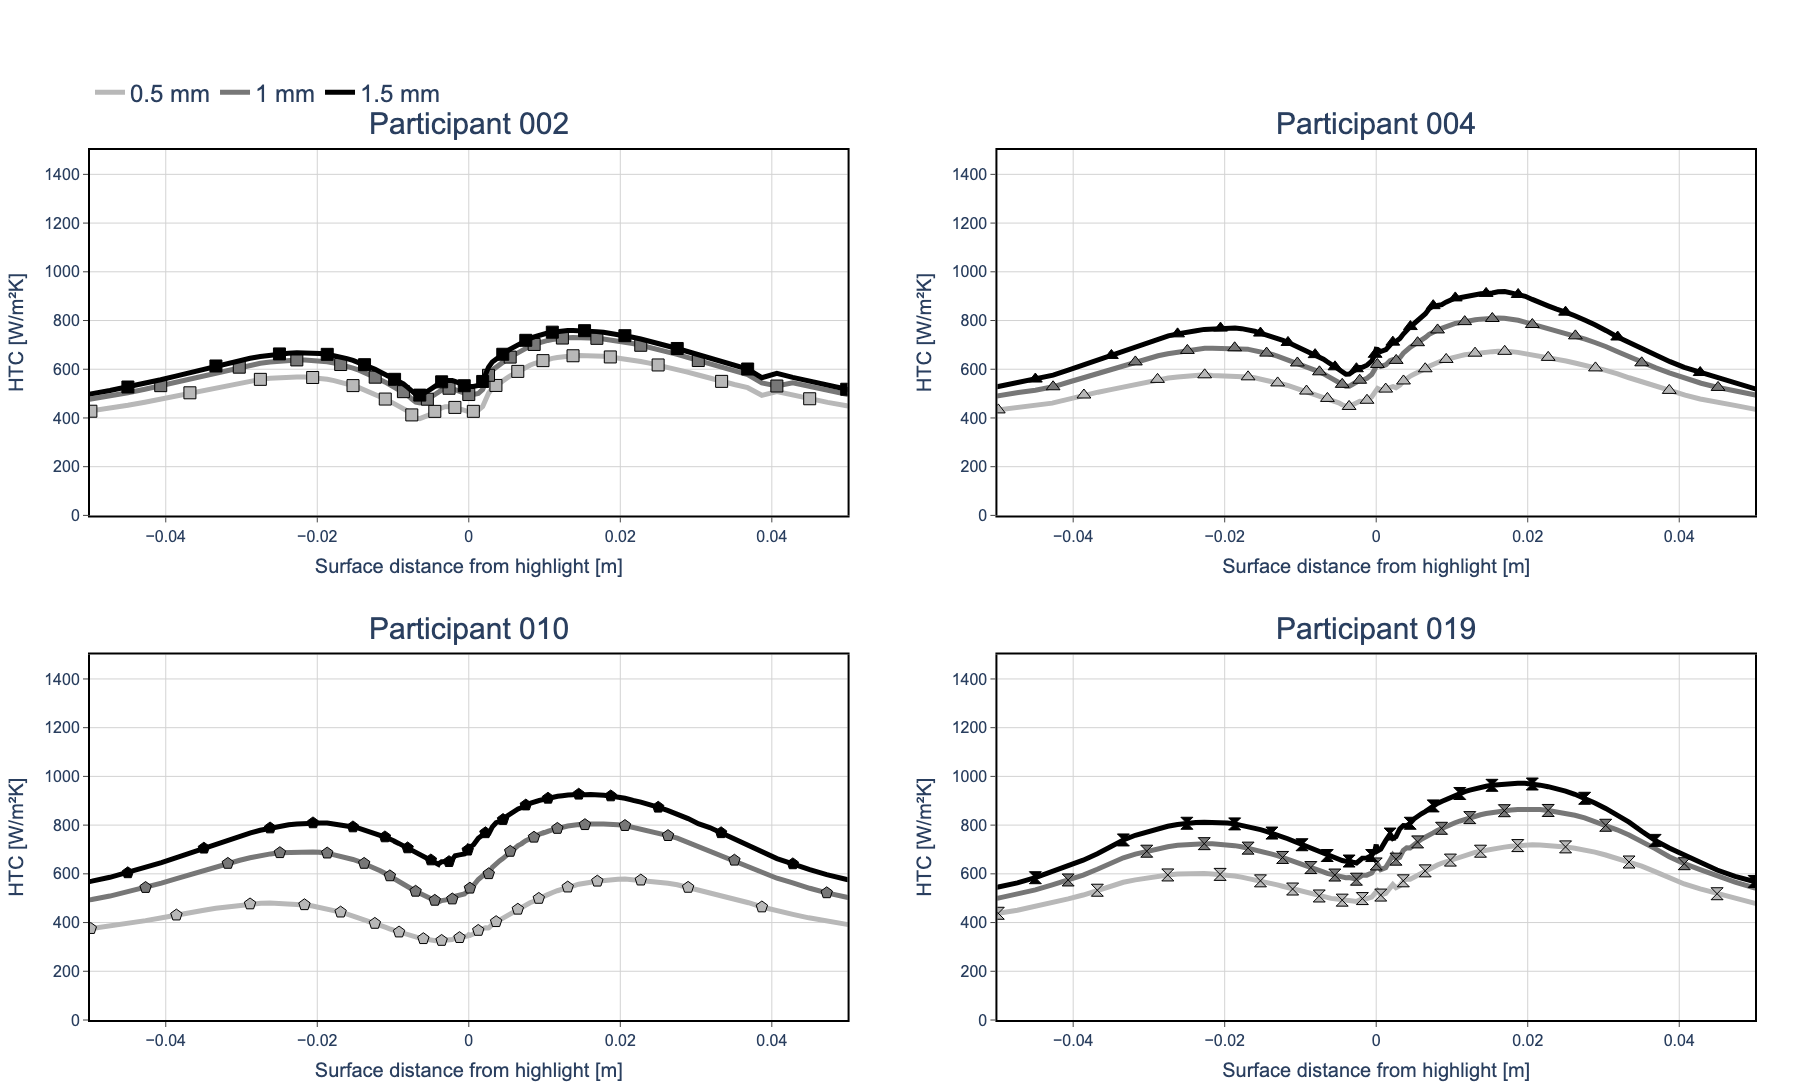
\includegraphics[width=0.8\textwidth]{FIGURES/HTC/tc_oneram6_L1_htc_vs_s_slice_0p1_all_roughness_participants.png}

\end{frame}

% ============================================================
% ============================================================
% END -- ONERA M6 CONVECTIVE HEAT TRANSFER
% ============================================================
% ============================================================
